\documentclass[11pt,twoside,a4paper]{report}
\usepackage{appendix}
\usepackage{geometry}
\usepackage{graphicx}
\usepackage{pdfpages}

% set the default, standard, geometry
\geometry{left=25mm, right=25mm, top=25mm, bottom=25mm}

\setlength{\parskip}{\baselineskip}
\clubpenalty10000
\hyphenpenalty10000
\widowpenalty10000

\begin{document}

\title{ID2216 Developing Mobile Applications\\Assignment 4 Report}
\author{Rafael Aldana (rafaelap@kth.se)\\Vincent Delitz (delitz@kth.se)\\Ruth Eriksson (ruthe@kth.se)}
\date{\today}
\maketitle



\tableofcontents
\thispagestyle{empty}

%\listoffigures

%\listoftables

\renewcommand{\chaptername}{Assignment}
\setcounter{chapter}{1}


\chapter{App web service}
\label{assignment:app-web-service}

\section{App web service overview}

After we received first feedback from tester for our initial draft of the Android app, we aimed to make it more useful and handy by integrating some web services. We decided to use therefore the Google Maps API, Facebook API and the database technology SQLite. 

\begin{itemize}
\item The Facebook API was used in order to let users register with their Facebook account in our app, so that they do not necessarily need an extra account for our app. Furthermore, the Facebook API enables us to integrate in the future more and better personalized services for the user.

\item In order to display the location of the pick up place in a more convenient way, we make use of Google Maps API, so that the user can see where on the map the pick up place is located.

\item To store our data in a managable and clear manner, we use SQLite which is a database API optimised for Android applications.

\end{itemize}

\section{Developing tools}

We chose to use Android Studio for several reasons:

\begin{itemize}

\item It is built purposely for Android, while for example Eclipse was built to all-purpose IDE that can be used with any language and platform.

\item It has a really nice interface design perspective where one can view the interface one is are working on and its related components.

\item Compared to Eclipse it is a much smaller IDE, therefore it uses less RAM space and lower CPU speed, so we get a very stable performance with no crashing and unresponsiveness.

\end{itemize}

\section{Feedback}



\section{Conclusion and outlook}

\begin{appendices}

\chapter{Figures}
\label{appendix}

\thispagestyle{empty}

\newpage

\begin{figure}
	\centering
	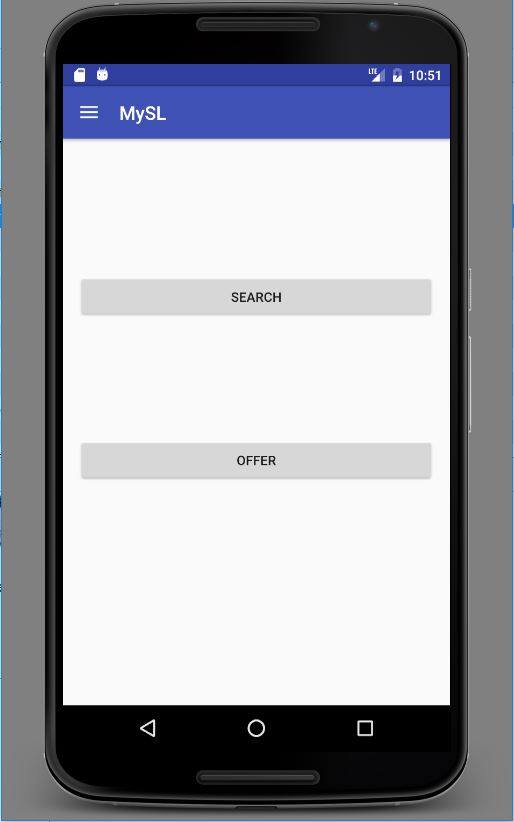
\includegraphics[width=0.4\textwidth]{jpg/android-start.jpg}
	\caption{Start view}
	\label{figure:start-view}
\end{figure}

\begin{figure}
	\centering
	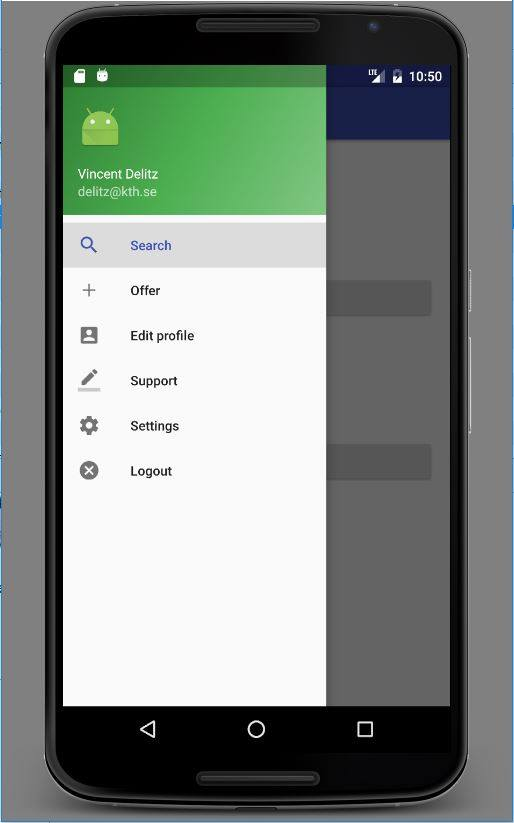
\includegraphics[width=0.4\textwidth]{jpg/android-navigation-drawer.jpg}
	\caption{Navigation drawer in start view}
	\label{figure:navigation-drawer-in-start-view}
\end{figure}

\begin{figure}
	\centering
	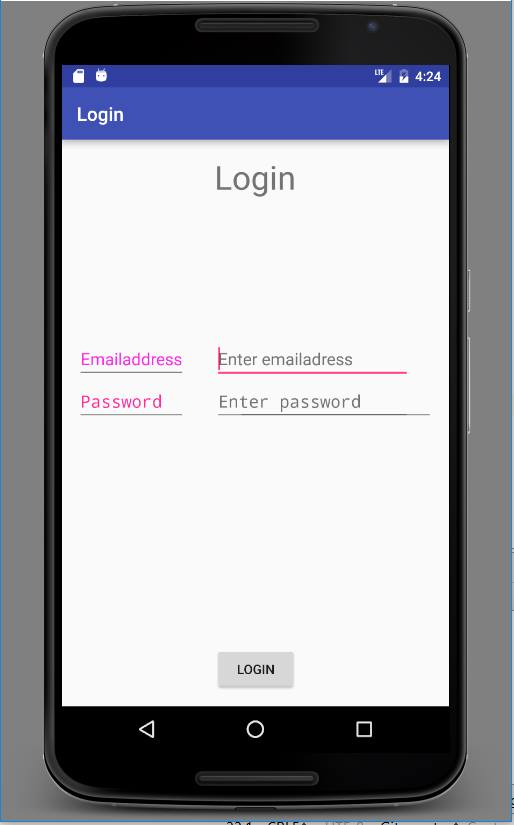
\includegraphics[width=0.4\textwidth]{png/android-login.png}
	\caption{Login view}
	\label{figure:navigation-drawer-in-start-view}
\end{figure}

\begin{figure}
	\centering
	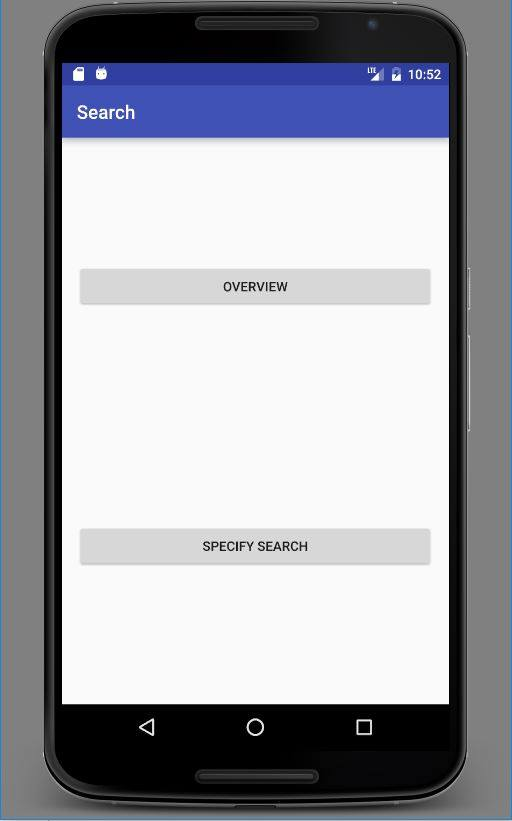
\includegraphics[width=0.4\textwidth]{jpg/android-search.jpg}
	\caption{Search view}
	\label{figure:search-view}
\end{figure}

\begin{figure}
	\centering
	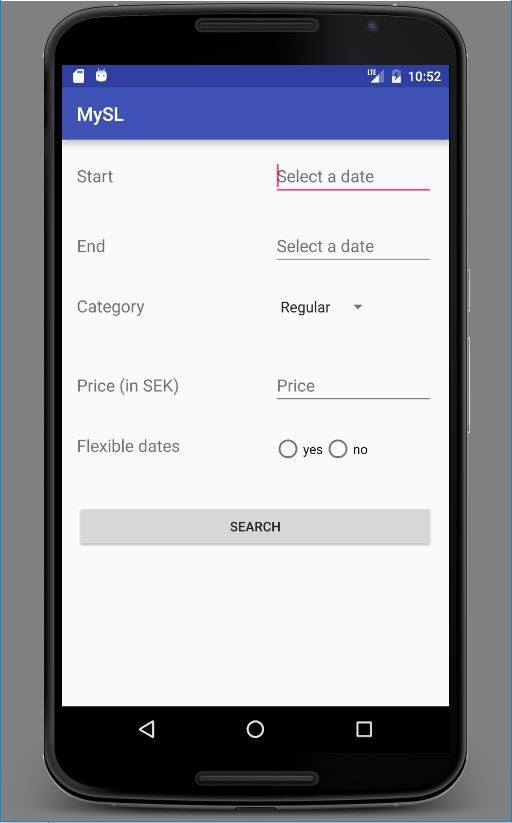
\includegraphics[width=0.4\textwidth]{jpg/android-specify-search.jpg}
	\caption{Specify search view}
	\label{figure:specify-search-view}
\end{figure}

\begin{figure}
	\centering
	\fcolorbox{black}{black}{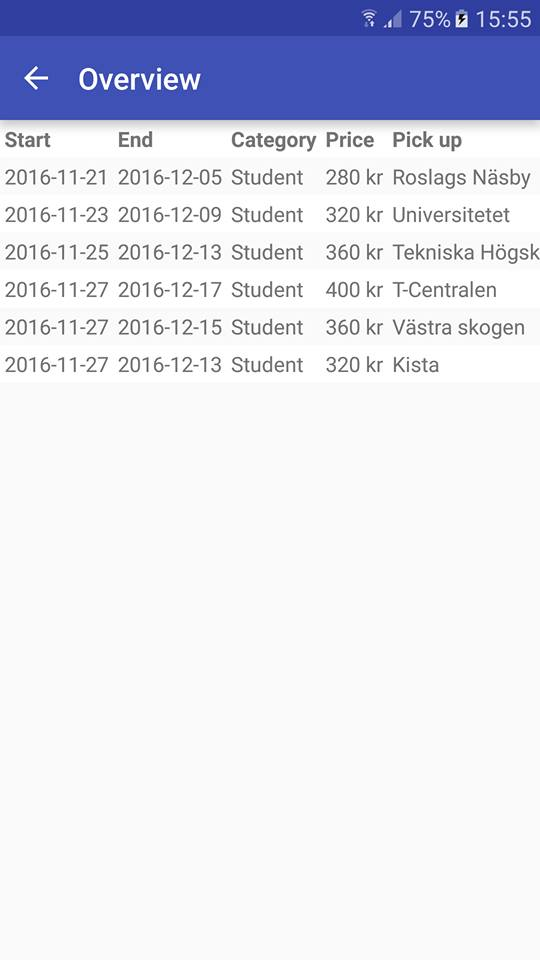
\includegraphics[width=0.4\textwidth]{png/android-overview.png}}
	\caption{Overview}
	\label{figure:overview}
\end{figure}

\begin{figure}
	\centering
	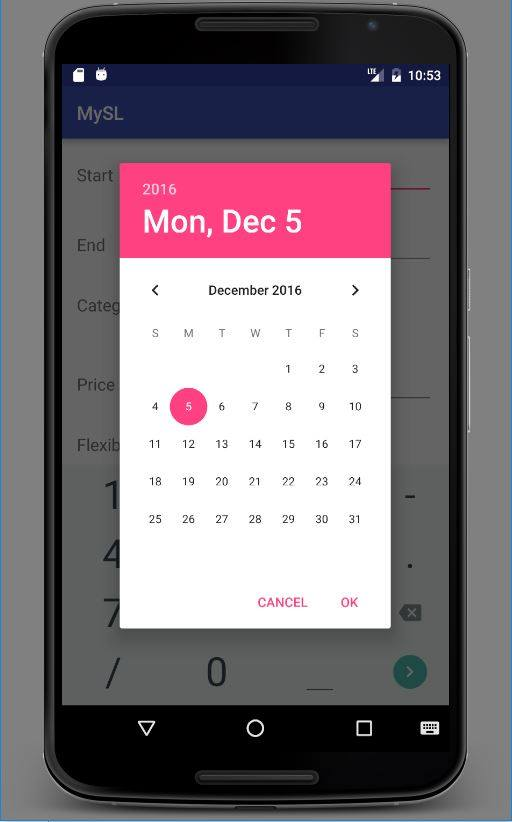
\includegraphics[width=0.4\textwidth]{jpg/android-calendar.jpg}
	\caption{Calendar view}
	\label{figure:calendar-view}
\end{figure}

\begin{figure}
	\centering
	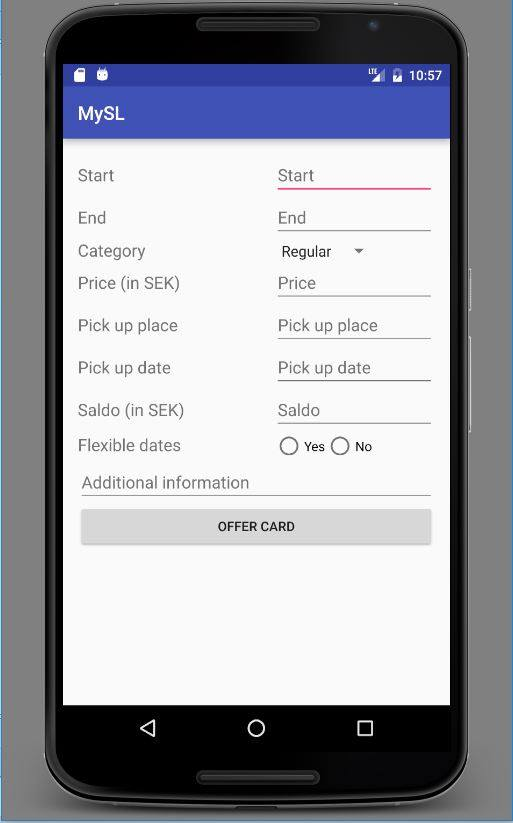
\includegraphics[width=0.4\textwidth]{jpg/android-offer.jpg}
	\caption{Offer view}
	\label{figure:offer-view}
\end{figure}

\end{appendices}

\end{document}